\chapter{Evolution II}

Key question: is evolution an experimentally testable theory?
\section{Case study: The Lenski Affair}

\begin{itemize}
    \item Starting at 1988, 12 identical cit- cultures (cit+ anaerobically) grew with limiting glucose and excess citrate.
    \item Dilute everyday and repeat freezing samples every 500 generations for about 30 years.
    \item In one culture only, weakly citrate-using (cit+) growth at generation about 31,500 is observed. And about 2000 more generations leads to strong cit+ growth.
    \item The experiment can be \textit{replayed} using the frozen samples.
\end{itemize}
This experiments provide evidence for potentiating mutation(s). It is an evolution under controlled laboratory conditions.

\section{Quiz 1: An always inherited gene}
\bd{Question} \\ [.1in]
How might we engineer an organism so that an altered gene (for flies) would always spread? \\ [.2in]
\bd{Solution} \\ [.1in]
Flies are complex organisms which \udl{reproduce sexually}. Each parent donates one chromosome from each of its pairs to the child. In this example the "red" gene is dominant in the sense that a single copy leads to the "red" phenotype.\\[.2in]
\bd{Normal inheritance}: the red fly has a "red" gene on one chromosome and a normal (blue) gene on the other as can be seen by the fact that it produces both red and blue children. If red flies always have to mate with blue flies, the red gene \udl{does not spread}.\\[.2in]
\bd{Gene drive inheritance}: the "red" gene \udl{drive gene copies} itself to the "blue" chromosome so that it is passed on to \textit{all} the children. This can be used in the lab to make mosquito populations sterile. This has not been tested in the wild, yet.
\begin{figure}[h]
\centering
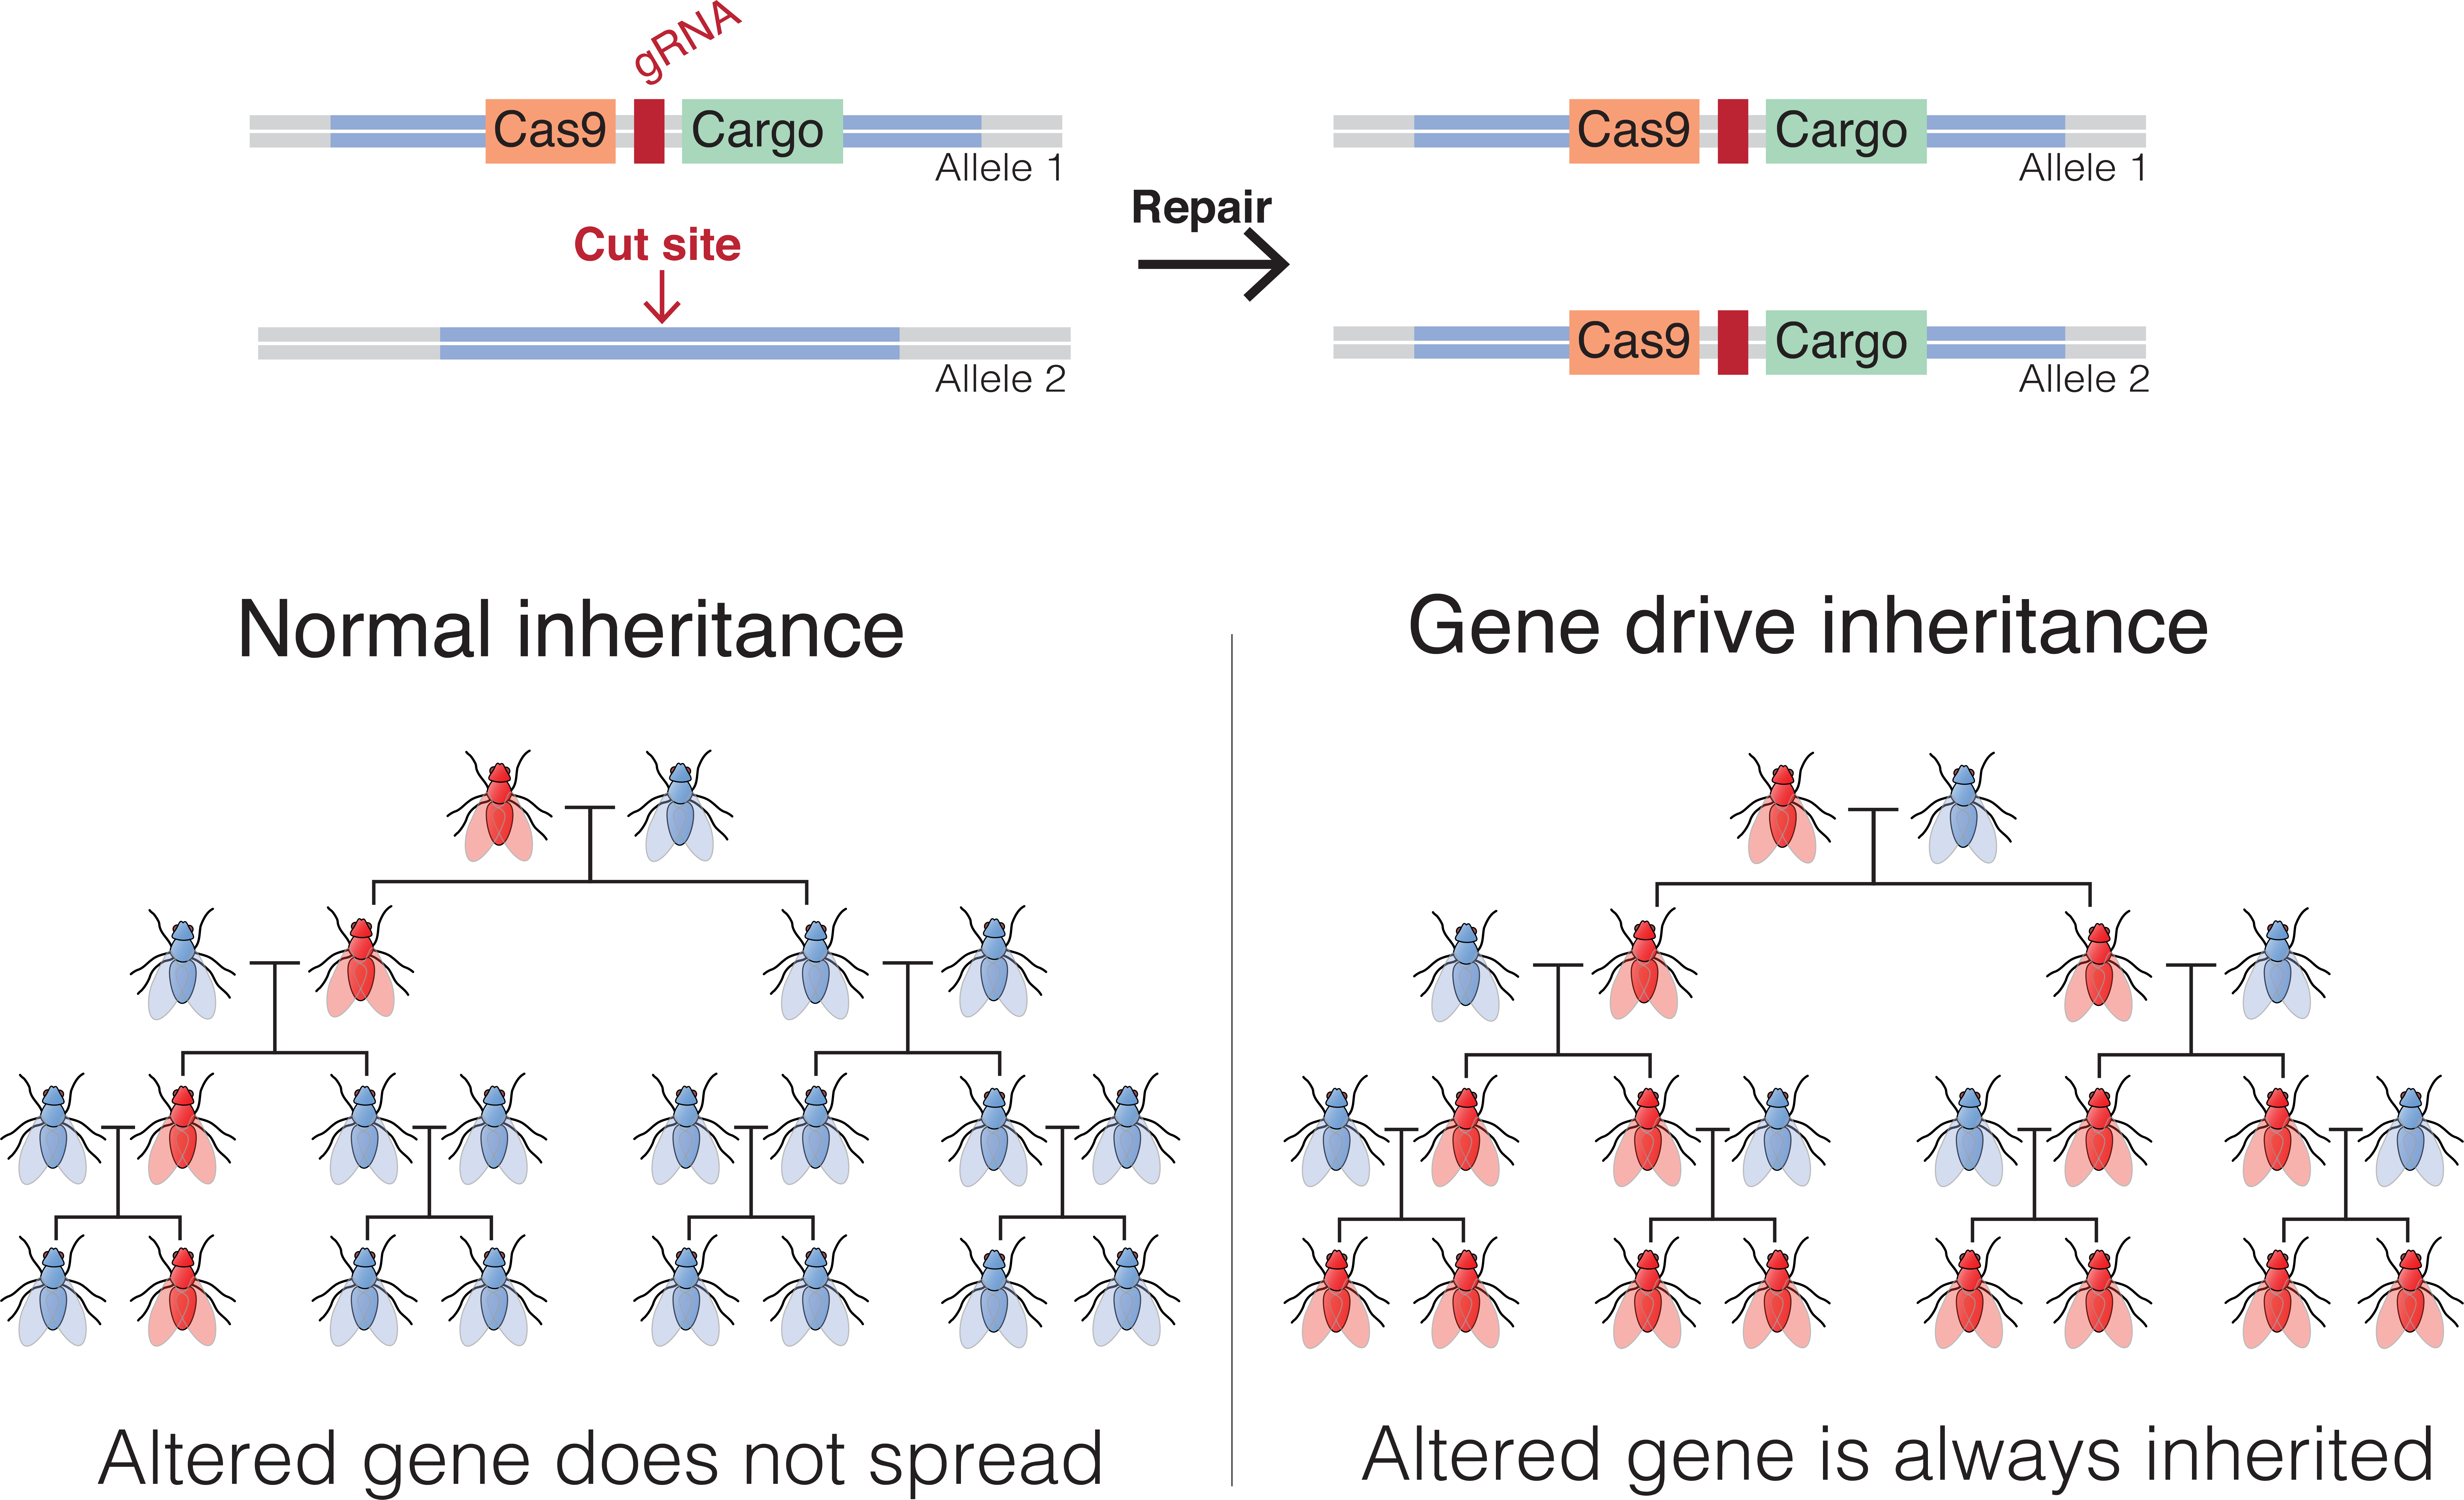
\includegraphics[width=1\textwidth]{images/Gene_Drive.png}\\[.2in]
\caption{Quiz 1 illustration} 
\end{figure}
\newpage
\section{Innate and Adaptive immune systems}
Both prokaryotes and eukaryotes have \udl{innate} and \udl{adaptive} \textit{immune systems} to protect them. These systems have provided excellent tools to bioengineers.
\begin{enumerate}
    \item \bd{Prokarotes}
    \begin{enumerate}
        \item \bd{Innate: Restriction enzymes}\\ Proteins that cut DNA at specific sequence (evolved to protect against viruses)
        \item \bd{Adaptive: CRISPR/cas9}\\ Programmable cutting of DNA, and more (evolved to protect against viruses)
    \end{enumerate}
    \item \bd{Eukaryotes}
    \begin{enumerate}
        \item \bd{Innate:} no typical example
        \item \bd{Adaptive: Antibodies}\\ Proteins that can bind to other molecules tightly and with high specificity (evolved to recognise pathogens\footnote{A bacterium, virus, or other microorganism that can cause disease.} and recruit responder cells)

    \end{enumerate}
\end{enumerate}
